\documentclass{beamer}
\usetheme{Madrid}
\usecolortheme{default}
\usepackage{amsmath}
\usepackage{graphicx}
\usepackage{algorithm}
\usepackage{algpseudocode}
\usepackage{setspace}
\usepackage{ragged2e}
\usepackage{booktabs}
\usepackage{lmodern}

% --- Meta Data ---
\title[ACDC for NIDS]{Automated Circuit Discovery for NIDS}
\subtitle{Mechanistic Interpretability for SOC-Oriented Security Research}
\author{Presented by: \textbf{Anbuselvi S}}

\begin{document}
	
	% Slide 1: Title
	\begin{frame}
		\titlepage
	\end{frame}
	
	% Slide 2: Outline
	\begin{frame}{Presentation Outline}
		\tableofcontents
	\end{frame}
	
	% --- SECTION 1: MOTIVATION ---
	\section{Motivation \& Background}
	
	% Slide 2
	\begin{frame}{The Interpretability Gap in NIDS}
		\begin{itemize}
			\setstretch{1.3}
			\item \justifying Modern NIDS use Deep Learning (Transformers/RNNs) for high accuracy.
			\item \justifying \textbf{The Black-Box Problem:} Analysts receive alerts but cannot verify the causal logic.
			\item \justifying \textbf{SOC Impact:} High false-positive rates and lack of trust in "AI-driven" security.
			\item \justifying \textbf{Solution:} Mechanistic Interpretability to reverse-engineer model internals.
			\item \justifying This motivates causal—not correlational—explanations.
		\end{itemize}
	\end{frame}
	
	% Slide 3
	\begin{frame}{Interpretability Methods in NIDS: A Comparison}
		\centering
		\scriptsize
		\renewcommand{\arraystretch}{1.75}
		
		\begin{tabular}{@{}p{2cm} p{2.5cm} p{2.1cm} p{3cm}@{}}
			\toprule
			\centering\textbf{Aspect} &
			\centering\textbf{Feature Attribution {\tiny (SHAP / LIME)}} &
			\centering\textbf{Rule-Based XAI} &
			\textbf{ACDC (Proposed)} \\
			\midrule
			
			Explanation Level &
			Input features &
			Human-defined rules &
			Internal computational components \\
			
			Causality &
			Correlational &
			Assumed by rules &
			Causal (via activation patching) \\
			
			Model Internals &
			Ignored &
			Not applicable &
			Explicitly analyzed \\
			
			Attack-Specific Logic &
			Weak &
			Manual &
			Automatically extracted \\
			
			SOC Usefulness &
			Limited &
			High but rigid &
			High and operationally actionable \\
			
			Forensic Value &
			Low &
			Moderate &
			High (circuit-level audit) \\
			
			\bottomrule
		\end{tabular}
	\end{frame}
	
	% Slide 4
	\begin{frame}{Applying ACDC to NIDS: Core Idea}
		\begin{itemize}
			\setstretch{1.3}
			\item In NIDS, the target behavior is an \textbf{attack detection decision}
			(e.g., SYN flood, scan, exfiltration).
			
			\item ACDC treats the trained NIDS as a \textbf{signal-processing system}
			that transforms raw traffic statistics into security decisions.
			
			\item The objective is to identify the \textbf{minimal internal computation}
			that maps:
			\begin{itemize}
				\item traffic patterns (rates, flags, temporal bursts)
				\item to an attack-specific alert.
			\end{itemize}
			
			\item The extracted circuit reveals \textbf{which traffic characteristics}
			and \textbf{which internal interactions} the NIDS truly relies on.
		\end{itemize}
	\end{frame}
	
	% --- SECTION 2: TECHNICAL FRAMEWORK ---
	\section{Technical Framework}
	
	% Slide 5
	\begin{frame}{Mapping ACDC Concepts to NIDS}
		\centering
		\small
		\renewcommand{\arraystretch}{1.5}
		\begin{tabular}{|p{3.5cm}|p{5.5cm}|}
			\hline
			\textbf{ACDC Concept} & \textbf{Interpretation in NIDS} \\
			\hline
			Behavior &
			Specific attack type (e.g., DDoS, Scan, Brute Force) \\
			\hline
			Computational Graph &
			NIDS model layers and feature interactions \\
			\hline
			Activation Patching &
			Replacing malicious traffic activations with benign baselines \\
			\hline
			Edge Pruning &
			Removing causally irrelevant feature pathways \\
			\hline
			Circuit &
			Minimal computation responsible for attack detection \\
			\hline
			Faithfulness Metric &
			KL divergence between full and pruned model outputs \\
			\hline
		\end{tabular}
	\end{frame}
	
	% Slide 6
	\begin{frame}{The NIDS Computational Graph}
		\begin{itemize}
			\setstretch{1.4}
			\item \justifying The trained NIDS is modeled as a \textbf{directed computational graph}.
			\vspace{0.3cm}
			\item \justifying \textbf{Nodes ($V$):} internal processing units such as
			feature interaction layers, temporal aggregation modules,
			attention heads, or hidden neurons.
			
			\item \justifying\textbf{Edges ($E$):} linear information pathways that propagate
			traffic signals (e.g., packet rates, flags, burst patterns)
			across the network.
			
			\item \justifying \textbf{Objective:} identify and retain only those edges that are	\textbf{causally necessary} for a specific attack detection behavior.
		\end{itemize}
		
		\vspace{0.4cm}
		\justifying This abstraction enables circuit discovery across different NIDS architectures
		(Transformer, RNN, CNN).
	\end{frame}
	
	
	% Slide 8
	\begin{frame}{System Architecture: ACDC-Enabled NIDS}
		\centering
		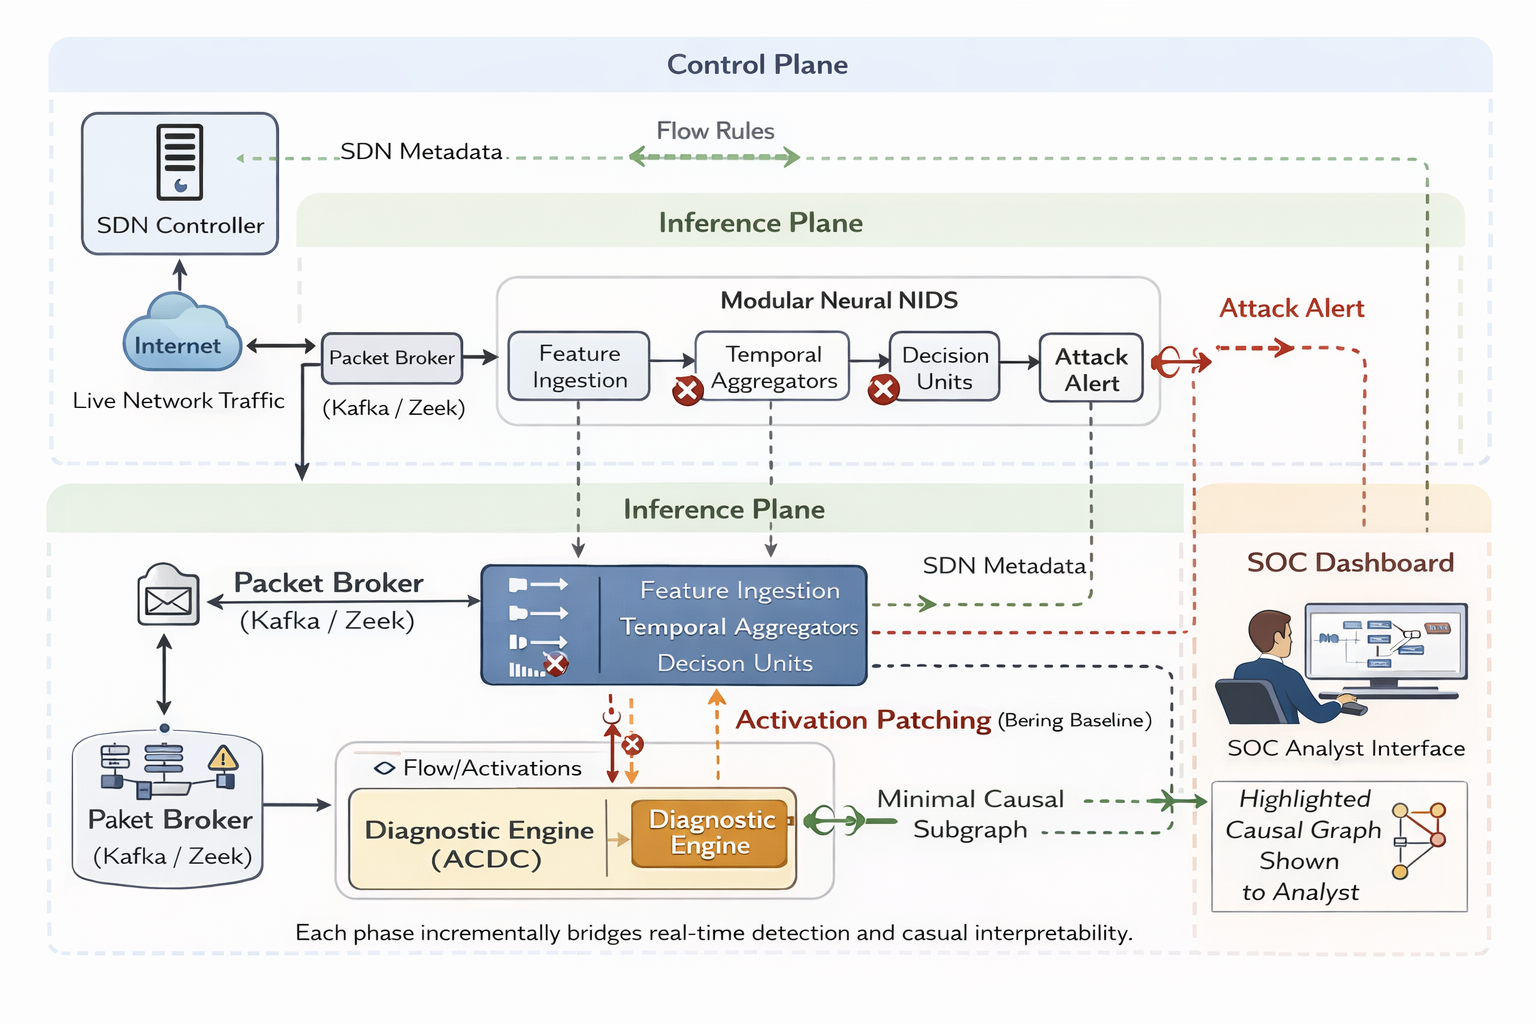
\includegraphics[width=1\textwidth]{1.png}
		
		%{\scriptsize
			%System architecture integrating deep learning NIDS with
			%ACDC-based circuit discovery}
	\end{frame}
	
	% Slide 9
	\begin{frame}{Step A: Task and Dataset Setup}
		To find a circuit, we must define the behavior:
		\vspace{0.5cm}
		\begin{block}{Task Definition}
			Detecting SYN Flood attacks within the UNSW-NB15 dataset.
		\end{block}
		\vspace{0.5cm}
		\begin{itemize}
			\item \textbf{Clean Dataset:} Malicious traffic samples.
			\item \textbf{Corrupted Dataset:} Normal baseline traffic or mean-ablated features.
		\end{itemize}
		\vspace{0.25cm}
		\justifying Behavior is quantified using the logit difference between Attack and Normal classes.
	\end{frame}
	
	% Slide 10
	\begin{frame}{Step B: Pruning Criterion ($\tau$)}
		ACDC removes an internal connection ($w \rightarrow v$) if it does not
		causally influence the attack detection outcome.
		
		\vfill
		\begin{equation*}
			D_{KL}(G \parallel H_{\text{new}}) - D_{KL}(G \parallel H) < \tau
		\end{equation*}
		\vfill
		
		\begin{itemize}
			\item \textbf{$G$}: Full NIDS model predicting attack vs. normal traffic.
			\item \textbf{$H$}: Current candidate circuit under evaluation.
			\item \textbf{$D_{KL}$}: Change in output probability distribution.
		\end{itemize}
		
		\vspace{0.4cm}
		KL divergence ensures the circuit preserves the \textbf{decision logic},
		not merely classification accuracy.
	\end{frame}
	
	\begin{frame}{Step C: Activation Patching}
		\begin{itemize}
			\setstretch{1.4}
			\item Internal activations from \textbf{corrupted (benign) traffic}
			are injected into the forward pass of \textbf{malicious traffic}.
			
			\item If the attack prediction remains unchanged, the patched
			connection is \textbf{not causally required} for detection.
			
			\item This allows ACDC to distinguish
			\textbf{true attack logic} from incidental correlations.
			
			\item \textbf{Example:} replacing SYN packet-rate activations
			with statistics from normal background traffic.
		\end{itemize}
	\end{frame}
	
	% --- SECTION 3: RESEARCH APPLICATIONS ---
	\section{Research Applications}
	
	% Slide 13
	\begin{frame}{Research: Generalization vs. Spurious Correlation}
		\begin{itemize}
			\setstretch{1.5}
			\item Does the NIDS learn \textbf{attack-relevant traffic patterns}
			(e.g., TCP flags, packet-rate bursts, temporal structure)?
			
			\item Or does it rely on \textbf{incidental identifiers}
			(e.g., source IPs, ports, or dataset-specific artifacts)?
			
			\item ACDC reveals whether the extracted circuit encodes
			\textbf{robust attack semantics} or shortcut-based correlations.
			
			\item This analysis helps distinguish \textbf{true generalization}
			from spurious detection behavior.
		\end{itemize}
	\end{frame}
	
	% Slide 14
	\begin{frame}{Example: Circuit Discovery for DDoS Detection}
		\begin{itemize}
			\setstretch{1.6}
			\item Consider a trained NIDS tasked with detecting \textbf{volumetric DDoS attacks}.
			
			\item ACDC isolates a \textbf{minimal detection circuit} that:
			\begin{itemize}
				\item aggregates packet-rate signals across short time windows,
				\item emphasizes sudden temporal traffic bursts,
				\item suppresses protocol-specific and benign background noise.
			\end{itemize}
			
			\item This circuit constitutes the \textbf{causal computation}
			sufficient for triggering a DDoS alert.
		\end{itemize}
	\end{frame}
	
	% Slide 15
	\begin{frame}{ACDC-Based Circuit Extraction for DDoS Attacks}
		\centering
		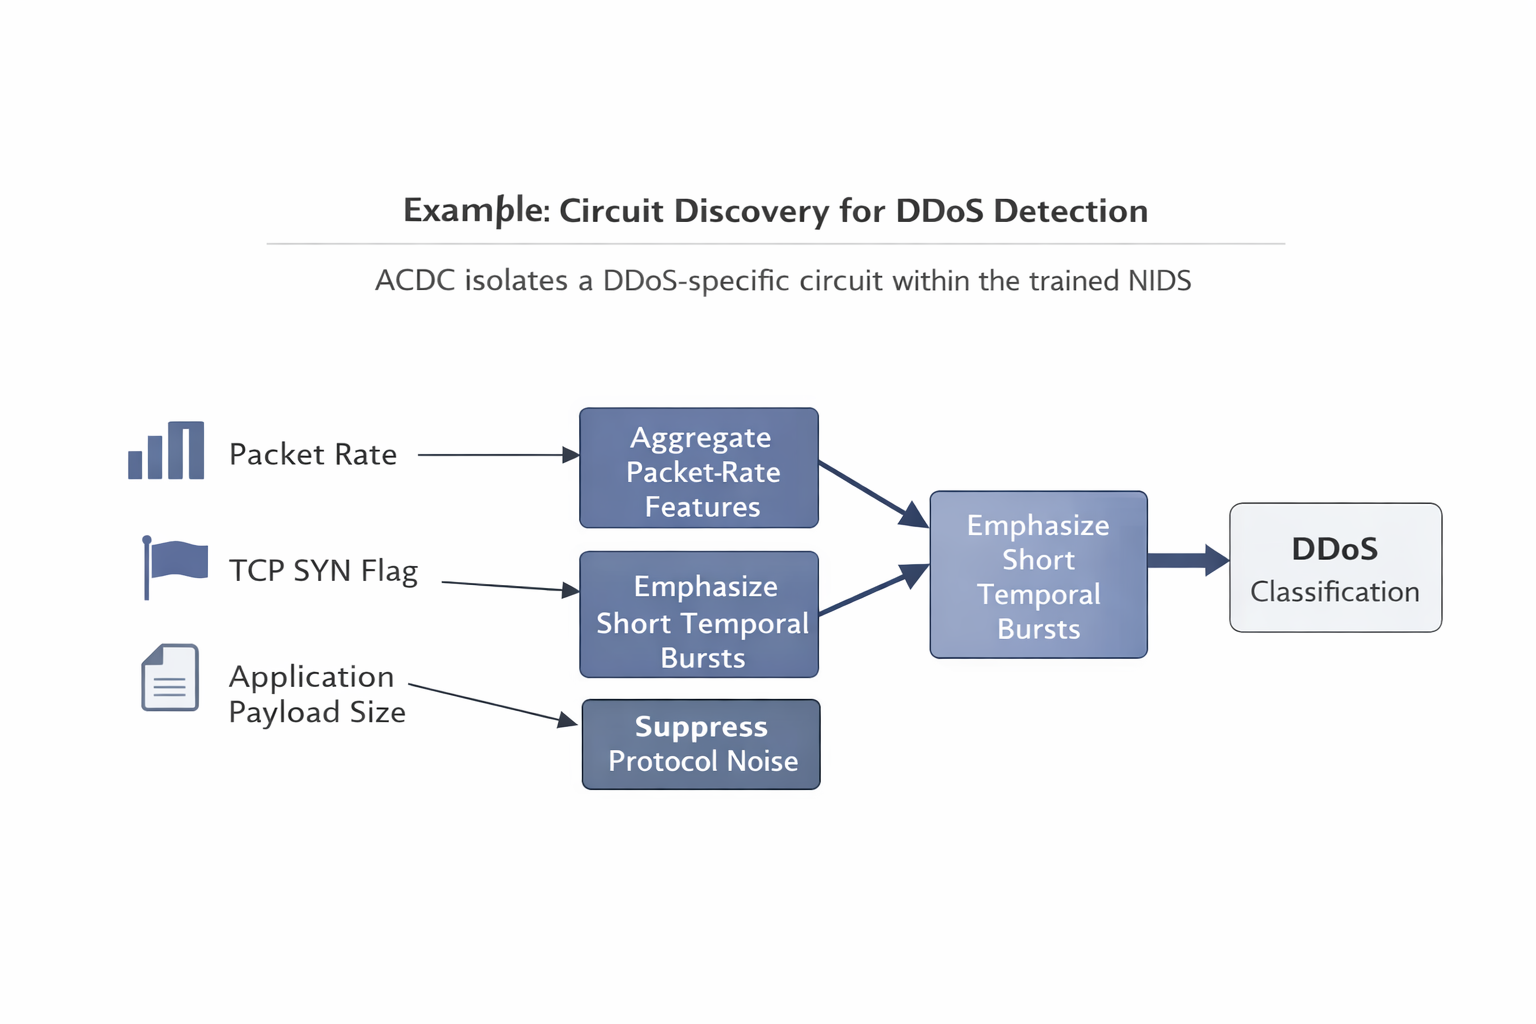
\includegraphics[width=1\textwidth]{4.png}
		
		{\scriptsize
			System architecture integrating deep learning NIDS with
			ACDC-based circuit discovery}
	\end{frame}
	
	% Slide 16
	\begin{frame}{Research: Adversarial Attack Resilience}
		\setstretch{1.6}
		\justifying
		
		\begin{itemize}
			\item Adversarial traffic can induce \textbf{pathway divergence},
			activating internal circuits normally associated with benign traffic.
			
			\item \textbf{Research Question:}
			To what extent can adversarial perturbations reroute computation
			away from the attack-specific circuit while preserving normal-traffic pathways?
			
			\item ACDC enables \textbf{circuit-level robustness analysis}
			by explicitly identifying which internal pathways are disrupted.
		\end{itemize}
	\end{frame}
	
	% Slide 17
	\begin{frame}{Technical Challenge: Scalability}
		\setstretch{1.5}
		\justifying
		
		\begin{itemize}
			\item Activation patching is computationally expensive
			for high-throughput network traffic.
			
			\item \textbf{Research Focus:}
			Attribution patching to approximate circuit importance
			with significantly reduced computational cost.
			
			\item As a result, ACDC is currently suited for
			\textbf{offline analysis and post-incident investigation},
			rather than inline detection.
		\end{itemize}
	\end{frame}
	
	% Slide 18
	\begin{frame}{Failure Case: The OR-Gate Problem}
		\begin{itemize}
			\setstretch{1.4}
			\item A NIDS may contain \textbf{redundant internal pathways}
			that independently support the same attack detection.
			
			\item If removing one pathway does not degrade detection performance,
			ACDC may incorrectly prune both during causal testing.
			
			\item This does not indicate model failure, but highlights
			\textbf{redundancy in the learned detection logic}.
			
			\item Addressing such redundancy remains an open research problem
			in circuit discovery methods.
		\end{itemize}
	\end{frame}	
	
	% --- SECTION 4: SOC OPERATIONS ---
	\section{SOC-Oriented Integration}
	
	% Slide 19
	\begin{frame}{System Design: ACDC-Enabled NIDS}
		\centering
		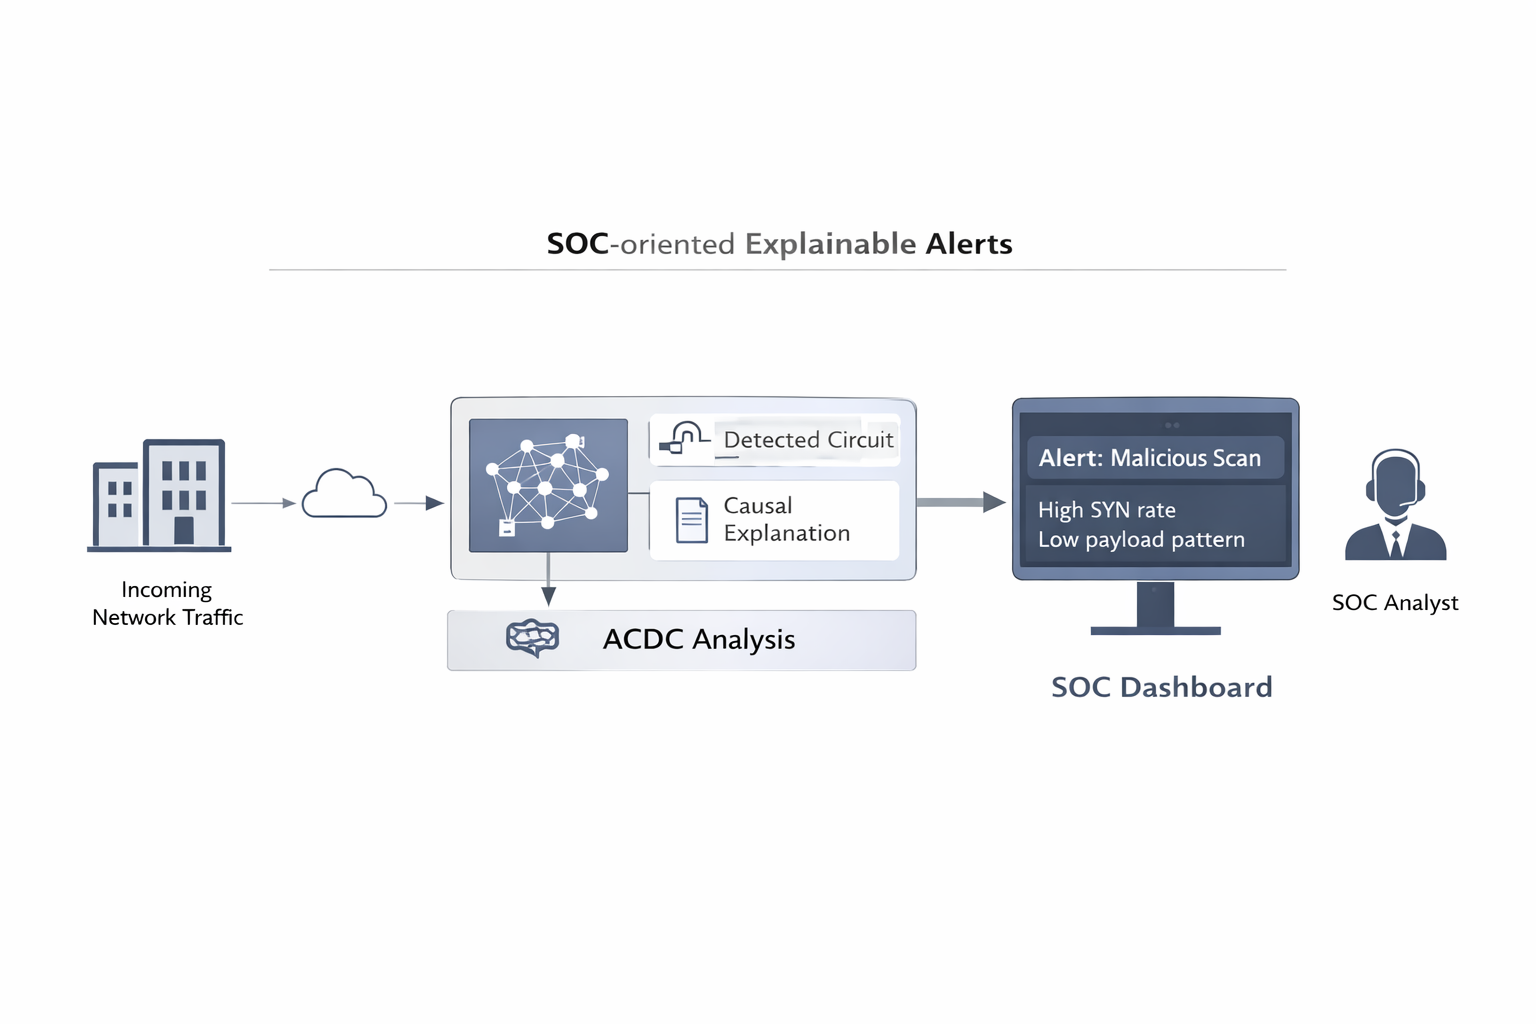
\includegraphics[width=1\textwidth]{3.png}
		
		{\scriptsize
			System architecture integrating deep learning NIDS with
			ACDC-based circuit discovery}
	\end{frame}
	
	% Slide 20
	\begin{frame}{SOC Integration: Transparent Alerts}
		Instead of: \textit{Alert: Anomaly detected}
		\vfill
		\begin{block}{ACDC-Enhanced Alert}
			Logic: Observed high SYN count combined with low data payload patterns.\\
			Causal confidence: 99.2\%.
		\end{block}
		\vspace{0.5cm}
		Circuits are summarized, not shown raw, to analysts.
	\end{frame}
	
	% Slide 21
	\begin{frame}{Automated Forensics for Tier-3 Analysts}
		\begin{itemize}
			\setstretch{1.3}
			\item For each detected attack, ACDC extracts the
			\textbf{internal detection circuit} used by the NIDS.
			
			\item Analysts can inspect the \textbf{behavioral logic}
			(e.g., traffic patterns and internal interactions)
			that triggered the alert.
			
			\item This supports \textbf{faster root-cause analysis}
			for advanced and previously unseen threats.
		\end{itemize}
	\end{frame}
	
	% Slide 22
	\begin{frame}{Logic-Based Filter Tuning and Evaluation}
		\begin{itemize}
			\setstretch{1.5}
			\item Circuit inspection identifies causes of false positives.
			\item Model refinement is applied only to implicated sub-components.
			\item Evaluation metrics:
			\begin{itemize}
				\setstretch{1.2}
				\item KL divergence under ablation,
				\item detection accuracy preservation,
				\item circuit sparsity.
			\end{itemize}
		\end{itemize}
	\end{frame}
	
	% Slide 23
	\begin{frame}{Building Operational Trust}
		\begin{itemize}
			\setstretch{1.4}
			\item \textbf{Auditability:}
			ACDC provides a causal explanation for each intrusion detection decision.
			
			\item \textbf{Accountability:}
			Enables post-incident review and justification in regulated and security-critical environments.
			
			\item \textbf{Inspectability:}
			Improves analyst confidence by making AI-driven decisions transparent rather than opaque.
		\end{itemize}
	\end{frame}	
	
	% --- SECTION 5: CONCLUSION ---
	\section{Conclusion}
	
	% Slide 14
	\begin{frame}{Summary}
		\begin{itemize}
			\setstretch{1.4}
			\justifying
			\item  Framed Network Intrusion Detection as a \textbf{mechanistic interpretability problem} rather than a black-box prediction task.
			
			\item Applied Automatic Circuit Discovery (ACDC) to extract \textbf{causal, attack-specific computational circuits} from trained NIDS models.
			
			\item Demonstrated how circuit-level explanations enable \textbf{auditable, trust-oriented decision support} for SOC operations.
		\end{itemize}	
	\end{frame}
	
	% Slide 25
	\begin{frame}{Future Directions}
		\begin{itemize}
			\setstretch{1.5}
			\item \justifying Scalable and approximate ACDC methods for high-speed network environments.
			\item Circuit discovery under redundancy and overlapping attack logic.
			\item Circuit-to-rule translation for deployment in SOC workflows.
			\item Behavioral analysis of zero-day attacks using circuit-level explanations.
			\item Human-in-the-loop refinement of interpretability for trusted NIDS.
		\end{itemize}
	\end{frame}
	
	\begin{frame}
		\centering
		\Large Thank You!
	\end{frame}
	
\end{document}
